% !TeX root = ./Serie03-JoelZuber-YannikDaellenbach.tex
% Gegeben seien die folgenden Anforderungen an einen Benutzer-System-Dialog:
% Ein Benutzer soll sich mit seinem Benutzernamen und seinem Passwort anmelden können. 
% Hierzu hat er maximal drei Versuche. 
% Nach dem dritten erfolglosen Versuch wird sein Konto gesperrt. 
% Während dem gesamten Login Prozess kann der Benutzer jederzeit in einen Subdialog "Reset Password" wechseln 
% an dessen Ende er wieder in den Status "Login" wechseln kann. 
% Nach einem erfolgreichen Login sieht der Benutzer "Sicht A" auf das System. 
% Er kann beliebig zwischen dieser "Sicht A" und einer zweiten "Sicht B" hin- und herwechseln. 
% Aus beiden Sichten A und B ist ein direktes Logout vorgesehen 
% (danach landet der Benutzer auf einer speziellen Logout Ansicht).
%
% Skizzieren Sie ein State Transition Network (STN), 
% welches diesen Dialog möglichst genau abbildet 
% (den Subdialog "Reset Password" müssen Sie nicht detailliert modellieren).
\begin{figure}[H]
  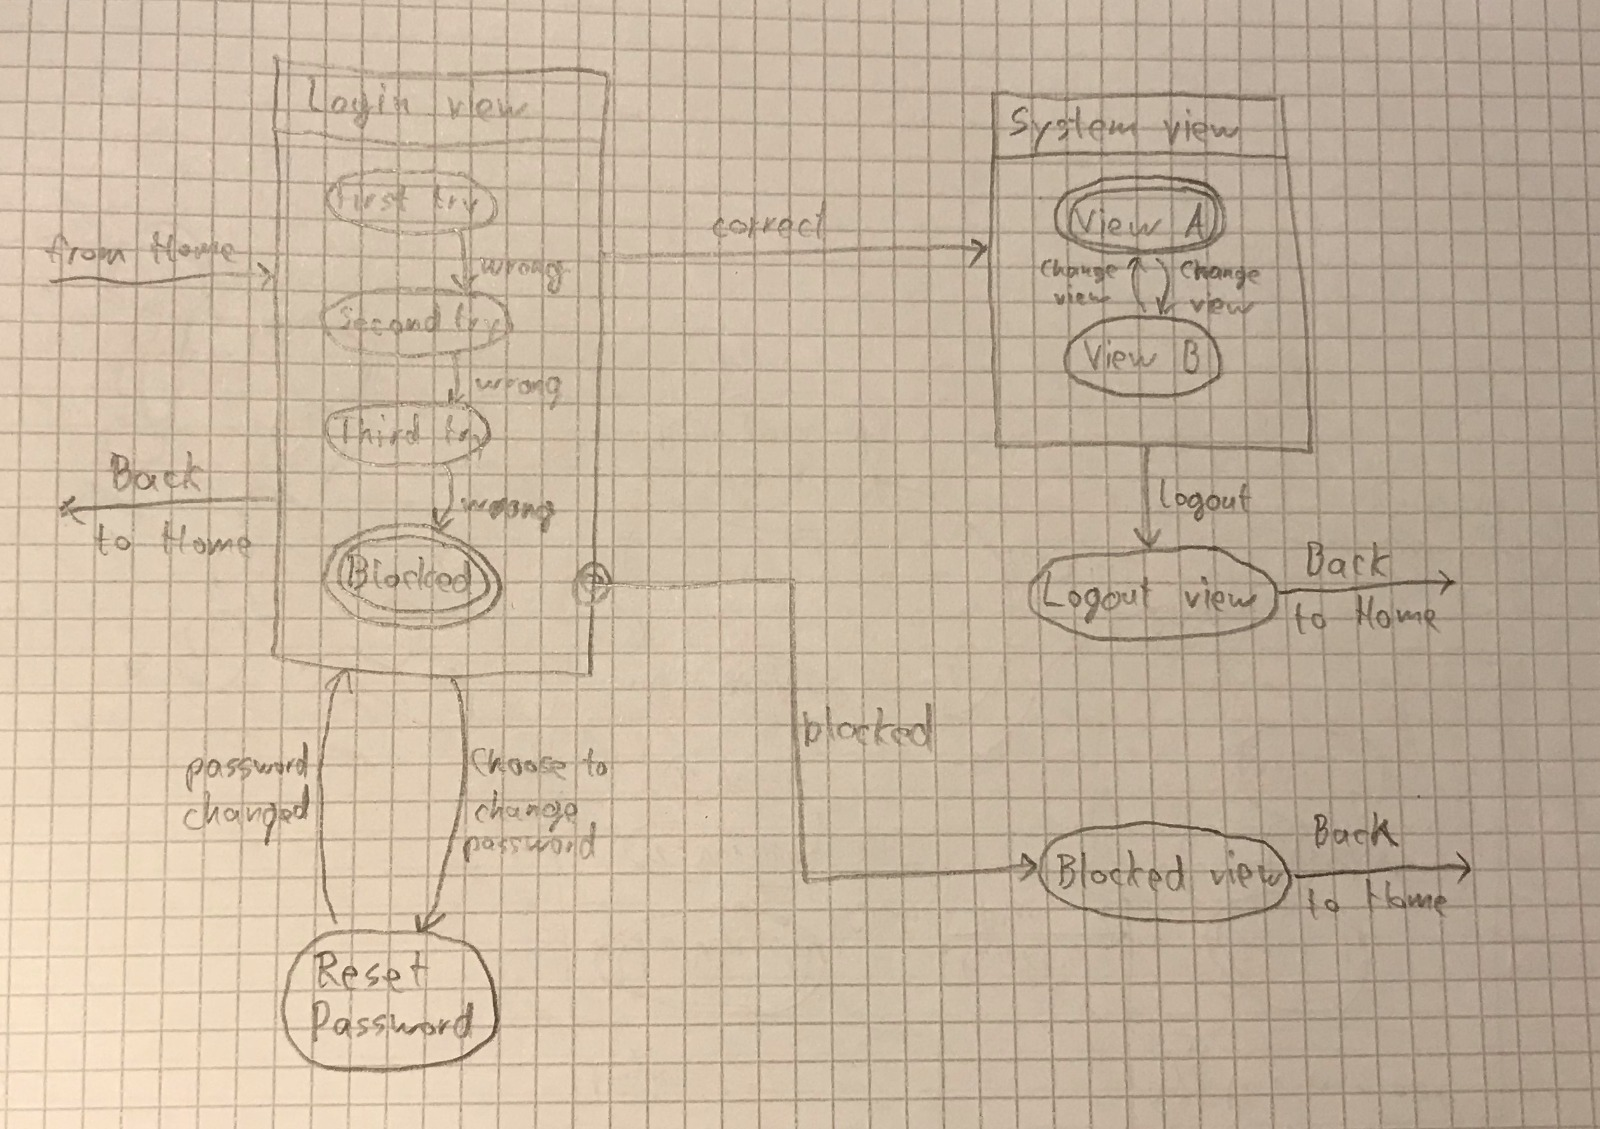
\includegraphics[width=\textwidth]{data/STN.jpeg}
  \caption{STN Login}
\end{figure}